\subsection{离散时间马氏链}

马尔可夫性 $\leftrightarrow$ 已知现在,过去与未来不相干/独立

\begin{definition}[(离散时间)马氏链]\label{def:M_1}
    称 $S$ 值随机过程 $\{X_n,n\geq 0\}$ 为马氏链,若 $X$ 满足以下马氏性:$\forall n\geq 0,x_0,x_1,\cdots,x_n,y\in S$,
    \[
    \PP(\underbrace{X_{n+1}=y}_{\text{未来}}|\underbrace{X_0=x_0,\cdots,X_{n-1}=x_{n-1}}_{\text{过去}},\underbrace{X_n=x_n}_{\text{现在}})=\PP(X_{n+1}=y|X_n=x_n)\tag{$M_1$}
    \]
    其中 $X_0$ 的分布称为 $X$ 的初始分布
\end{definition}

\begin{definition}
    当 $S$ 为有限集,称链为有限链,当 $S$ 为无限集,称链为无限链
\end{definition}

注:改写 $(M_1)$
\[
LHS=\PP_{X_n=x_n}(X_{n+1}=y|X_0=x_0,\cdots,X_{n-1}=x_{n-1})
\]
\[
RHS=\PP_{X_n=x_n}(X_{n+1}=y)
\]
\[
\begin{aligned}
    M_1 &\Leftrightarrow \{X_{n+1}=y\}\ind_{\{X_n=x_n\}}\{X_0=x_0,\cdots,X_{n-1}=x_{n-1}\}\\
    &\Leftrightarrow X_{n+1}\ind_{\{X_n=x_n\}} (X_0,\cdots,X_{n-1})
\end{aligned}
\]
$(M_1)\quad \text{未来}\ind_{\text{现在}}\text{过去}$
\[
\PP_{\text{现在}}(\text{未来}|\text{过去})=\PP_{\text{现在}}(\text{未来})
\]

\begin{lemma}[马氏性的等价表示]
    [G S] 下面三个命题等价
    \begin{enumerate}
        \item $(M_1)$ 马氏性
        \item $\forall k\geq 0, 0\leq n_1< \cdots<n_k\leq n$,对于 $y,x_{n_1},\cdots,x_{n_k}\in S$,
        \[
        \PP(X_{n+1}=y|X_{n_1}=x_{n_1},\cdots,X_{n_k}=x_{n_k})=\PP(X_{n+1}=y|X_{n_k}=x_{n_k})\tag{$M_2$}
        \]
        即
        \[
        \{X_{n+1}=y \}\ind_{\{X_{n_k}=x_{n_k}\}}\{X_{n_1}=x_{n_1},\cdots,X_{n_{k-1}}=x_{n_{k-1}}\}
        \]
        \item 对 $\forall m\geq 1,n\geq 0, \{y,x_i,0\leq i\leq n\}\st S$,有
        \[
        \PP(X_{n+m}=y|X_0=x_0,\cdots,X_n=x_n)=\PP(X_{n+m}=y|X_n=x_n)\tag{$M_3$}
        \]
        即
        \[
        \{X_{n+m}=y\}\ind_{\{X_n=x_n\}}\{X_0=x_0,\cdots,X_{n-1}=x_{n-1}\}
        \]
    \end{enumerate}
\end{lemma}

证明:$(2)\rightarrow (1)$,取 $n_1=0,\cdots,n_k=n-1$,显然

$(2)\rightarrow (3)$,(3)的$n$对应(2)的$n_k$

$(3)\rightarrow (1)$ 显然

只需证 $(3)\rightarrow (2),(1)\rightarrow (3)$

这里回顾独立的三种写法
\begin{enumerate}
    \item $A\ind_B C$ 记号
    \item $\PP_B(A,C)=\PP_B(A)\PP_B(C)$ 定义
    \item $\PP_B(A|C)=\PP_B(A)$ 定理
\end{enumerate}

(Step 1) 证明 $(3)\rightarrow (2)$

对 $\forall k\geq 2, 0\leq n_1<n_2<\cdots<n_k=n$

令 $J=\{0,1,\cdots,n_k\}\backslash \{n_1,\cdots,n_k\}$, $\tilde{\PP}(\cdot)=\PP(\cdot|X_{n_1}=x_{n_1},\cdots,X_{n_k}=x_{n_k})$

\[
\begin{aligned}
    \tilde{\PP}(X_{n+1}=y)&=\sum_{x_j\in S,j\in J}\cdot\tilde{\PP}(X_{n+1}=y|X_j=x_j,j\in J)\tilde{\PP}(X_j=x_j,j\in J)\qquad [\text{全概公式}]\\
    &=\PP(X_{n+1}=y|X_{n_k}=x_{n_k})\sum_{x_j\in S,j\in J}\tilde{\PP}(X_j=x_j,j\in J)\qquad [(3), \PP_C(\cdot|A)=\PP_C(\cdot)]\\
    &=\PP(X_{n+1}=y|X_{n_k}=x_{n_k})
\end{aligned}
\]

其中,记号 $\sum_{x_j\in S,j\in J}$ 中的下标意为:假设 $J$ 中元素个数为 $\# J=u$,则 $(x^{(1)},\cdots, x^{(u)})\in S^u$。从简单的开始,$\sum_{x\in S}\PP(X=x)=\PP(\Omega), \sum_{(x,y)\in S^2}\PP(X=x,Y=y)=\PP(\Omega),\cdots$,$\sum_{(x^{(1)},\cdots, x^{(u)})\in S^u}\PP(X^{(1)}=x^{(1)},\cdots,X^{(u)}=x^{(u)})=\PP(\Omega)=1$

(Step 2) 下证 $(1)\rightarrow (3)$

1. $m=1$ 时,即 $(1)$

2. 假设 $m=k$ 时 $(3)$ 成立,即 $\forall n\geq 1, \{y,x_i,n\geq i\geq 0\}\st S$,
\[
\{X_{n+k}=y\}\ind_{\{X_n=x_n\}}\{X_0=x_0,\cdots, X_{n-1}=x_{n-1}\}\xrightarrow{\text{作业}}\{X_{n+k}=y\}\ind_{\{X_n=x_n\}}\{X_{n-1}=x_{n-1}\}
\]
\[
\begin{aligned}
    \PP(X_{n+k}=y|X_0=x_0,\cdots,X_n=x_n)&=\PP(X_{n+k}=y|X_n=x_n)\\
    &=\PP(X_{n+k}=y|X_n=x_n,X_{n-1}=x_{n-1})
\end{aligned}\tag{*}
\]
当 $m=k+1$ 时,对 $\forall \{y,x_i,n\geq i\geq 0\}\st S$

令 $\tilde{\PP}_n(\cdot):=\PP(\cdot|X_0=x_0,\cdots,X_n=x_n)$
\[
\begin{aligned}
    \tilde{\PP}_n(X_{n+k+1}=y)&=\sum_{x_{n+1}\in S}\tilde{\PP}_n(X_{n+k+1}=y|X_{n+1}=x_{n+1})\cdot \tilde{\PP}_n(X_{n+1}=x_{n+1})\\
    &=\sum_{x_{n+1}\in S}\PP(X_{n+k+1}=y|X_{n+1}=x_{n+1},X_n=x_n)\cdot \PP(X_{n+1}=x_{n+1}|X_n=x_n)\qquad [\text{by (*)}]\\
    &=\sum_{x_{n+1}\in S}\PP(X_{n+k+1}=y,X_{n+1}=x_{n+1},X_n=x_n)/\PP(X_n=x_n)\qquad [\text{乘法公式-定理\eqref{thm:multiply_func}}]\\
    &=\sum_{x_{n+1}\in S}\PP(X_{n+k+1}=y,X_n=x_n)/\PP(X_n=x_n)\\
    &=\sum_{x_{n+1}\in S}\PP(X_{n+k+1}=y|X_n=x_n)
\end{aligned}
\]
即 $m=k+1$ 得证\qed

\begin{corollary}\label{cor:markov_con_cut}
    若 $X$ 时马氏链,则 $\forall n\geq 1,\{x_i,n\geq i\geq 0,y\}\st S$,有 
    \[
    \PP(X_{n+1}=y|X_0=x_0,\cdots,X_n=x_n)=\PP(X_{n+1}=y|X_n=x_n,X_{n-1}=x_{n-1})
    \]
\end{corollary}

补充记号:
\begin{itemize}
    \item 乘积空间
    \[
        S^n:=\underbrace{S\times\cdots\times S}_{\text{n个}}
    \]
    \item 乘积 $\sigma$ 代数
    \[
        \bigotimes_n 2^S:=\underbrace{2^S\times\cdots\times 2^S}_{\text{n个}}
    \]
\end{itemize}

\begin{property}[马氏性的等价条件]
下列三个命题等价
\begin{enumerate}
    \item 马氏性 $(M_1)$
    \item 对 $\forall n\geq 1,m\geq 1,A\in \otimes_n 2^S,B\in \otimes_m 2^S$,即 $(A\st S^n,B\st S^m)$,有
    \[
    \begin{aligned}
        &\PN((X_0,\cdots,X_{n-1})\in A,(X_{n+1},\cdots,X_{n+m})\in B)\\
        =&\PN((X_0,\cdots,X_{n-1})\in A)\cdot \PN((X_{n+1},\cdots,X_{n+m})\in B)
    \end{aligned}
    \]
    即 $(X_0,\cdots,X_{n_1})\ind_{\{X_n=x_n\}}(X_{n+1},\cdots,X_{n+m})$ 的定义
    \item $\PN((X_{n+1},\cdots,X_{n+k+1})\in B|(X_0,\cdots,X_{n-1})\in A)=\PN((X_{n+1},\cdots,X_{n+k+1})\in B)$
\end{enumerate}
\end{property}

证明:$(2)\Leftrightarrow (3)$,独立的定义和定理,显然

$(3)\rightarrow (1)$,取 $k=0$ 显然

只需证 $(1)\rightarrow (3)$

只需证 $(3)$ 对简单事件 $A,B$ (单点集合) 成立,即 $\forall n\geq 1,m\geq 1, \{x_0,x_1,\cdots,x_{n+m}\st S\}$,有
\[
\PN((X_{n+1},\cdots,X_{n+m})=x_{n+1}^{n+m}|(X_0,\cdots,X_{n-1})=x_0^{n-1})=\PN((X_{n+1},\cdots,X_{n+m})=x_{n+1}^{n+m})
\]
其中 $x_{n+1}^{n+m}=(x_{n+1},\cdots,x_{n+m}),x_{n+1}^{n+m}=(x_0,\cdots,x_{n-1})$

*只要对单点集合成立,对一般情况也成立,证明见独立性部分

只证 $m=2$,令
\[
\tilde{\PP}_n(\cdot):=\PN(\cdot|(X_0,\cdots,X_{n-1})=x_0^{n-1})=\PP(\cdot|(X_0,\cdots,X_{n})=x_0^{n})
\]
$\Rightarrow$
\[
\begin{aligned}
    \tilde{\PP}_n((X_{n+1},X_{n+2})=(x_{n+1},x_{n+2}))&=\tilde{\PP}_n(X_{n+1}=x_{n+1})\cdot \tilde{\PP}_n(X{n+2}=x_{n+2}|X_{n+1}=x_{n+2})\\
    &=\PP(X_{n+1}=x_{n+1}|X_n=x_n)\cdot \PP(X_{n+2}=x_{n+2}|X_{n+1}=x_{n+1})\qquad [M_1]\\
    &=\PP(X_{n+1}=x_{n+1}|X_n=x_n)\cdot \PP(X_{n+2}=x_{n+2}|X_{n+1}=x_{n+1},X_n=x_n)\qquad [\text{推论\eqref{cor:markov_con_cut}}]\\
    &=\PN(X_{n+1}=x_{n+1})\cdot \PN(X_{n+2}=x_{n+2}|X_{n+1}=x_{n+1})\\
    &=\PN((X_{n+1},X_{n+2})=(x_{n+1},x_{n+2}))\qquad [\text{乘法公式-定理\eqref{thm:multiply_func}}]
\end{aligned}
\]

\begin{corollary}
    设 $X$ 为马氏链,则对每一个 $n\geq 1,m\geq 1, u_k<u_{k+1}, 0\leq k\leq n+m-1$,有
    \[
    (X_{u_0},\cdots,X_{u_{n-1}})\ind_{\{X_{u_n}=x_{u_n}\}}(X_{u_{n+1}},\cdots,X_{u_{n+m}})
    \]
\end{corollary}

\subsection{时齐马氏链与转移概率}

\begin{definition}[时间齐次马氏链]
    称马氏链 $X:\{X_n,n\geq 0\}$ 为时齐的或时间齐次马氏链,若对 $\forall n\geq 0, i,j\in S$
    \[
    \PP(X_{n+1}=j|X_n=i)=\PP(X_1=j|X_0=i)
    \]
\end{definition}

\begin{definition}
    $X$ 是时齐马氏链,称
    \[
    p_{ij}:=p_{i,j}=\PP(X_1=j|X_0=i)\qquad i,j\in S
    \]
    为 $X$ 从状态 $i$ 到 $j$ 的(一步)\textbf{转移概率},并称矩阵
    \[
    P=\begin{pmatrix}
        p_{11} & p_{12} & p_{13} & \cdots\\
        p_{21} & p_{22} & p_{23} & \cdots\\
        \vdots & \vdots & \vdots & \ddots
    \end{pmatrix}
    \]
    为(一步)转移(概率)矩阵
\end{definition}

若不加说明,则默认讨论的马氏链都是时齐的

注:
\[
\begin{aligned}
    \PP(x_{n+1}=y)&=\sum_{x\in S}\PP(X_{n+1}=y|X_n=x)\cdot \PP(X_n=x)\\
    &=\sum_{x\in S}p_{xy}\cdot \PP(X_n=x)
\end{aligned}
\]

\begin{theorem}[转移矩阵的刻画]
    转移矩阵是一个随机矩阵,即
    \begin{enumerate}
        \item $\forall i,j\in S,p_{ij}\geq 0$
        \item $\forall i\in S,\sum_{j\in S}p_{ij}=1$
    \end{enumerate}
    即转移矩阵的每一行 $(p_{ij})_{j\in S}$ 为 $S$ 上的一个概率分布

    注:另一种随机矩阵是指元素为随机变量的矩阵,和这里讲的没有关系
\end{theorem}

证明:
\[
\sum_{j\in S}\PP(X_1=j|X_0=i)=\PP(X_1\in S|X_0=i)=\PP(\Omega|X_0=i)=1
\]

\begin{definition}[时齐马氏链]\label{def:homo-markov}
    设 $X=\{X_n,n\geq 0\}$ 为一随机过程,若
    \begin{enumerate}
        \item 初值 $X_0$ 满足分布 $\mu=(\mu_i)_{i\in S}$,即 $\PP(X_0=i)=\mu_i,i\in S$
        \item 存在一个随机矩阵 $P=(p_{ij})_{i,j\in S}$ 使得 $\forall n\geq 1,i_n,\cdots,i_{n-1},i,j\in S$
        \[
        \PP(X_{n+1}=j|X_0=i_0,\cdots,X_{n-1}=i_{n-1},X_n=i)=p_{ij}
        \]
    \end{enumerate}
    则称 $X$ 具有初始分布 $\mu$ 和转移矩阵 $P$ 的(时齐)马氏链,记作 $X\sim \text{Markov}(\mu,P)$
\end{definition}

上述定义与$(M_1)$马氏链定义\ref{def:M_1}等价

证明:$(2)\rightarrow (M_1)$
\[
\PN(X_{n+1}=j)=\sum_{(i_0,\cdots,i_{n-1})\in S^n}\PN (X_{n+1}=j|X_0=i_0,\cdots,X_{n-1}=i_{n-1})
\]
\[
\PN(X_0=i_0,X_{n-1}=i_{n-1})\overset{(2)}{=}p_{ij}\sum_{(i_0,\cdots,i_{n-1})\in S^n}\PP(X_0=i_0,\cdots,X_{n-1}=x_{n-1}|X_n=i)=p_{ij}
\]
即然有 $(M_1)$,为什么还要定义\ref{def:homo-markov}?因为该定义决定了马氏链的有限维分布

\begin{example}[Gambler's Ruin]
    [Durrett, 3rd ed] P1 
    \begin{figure}[H]
        \centering
        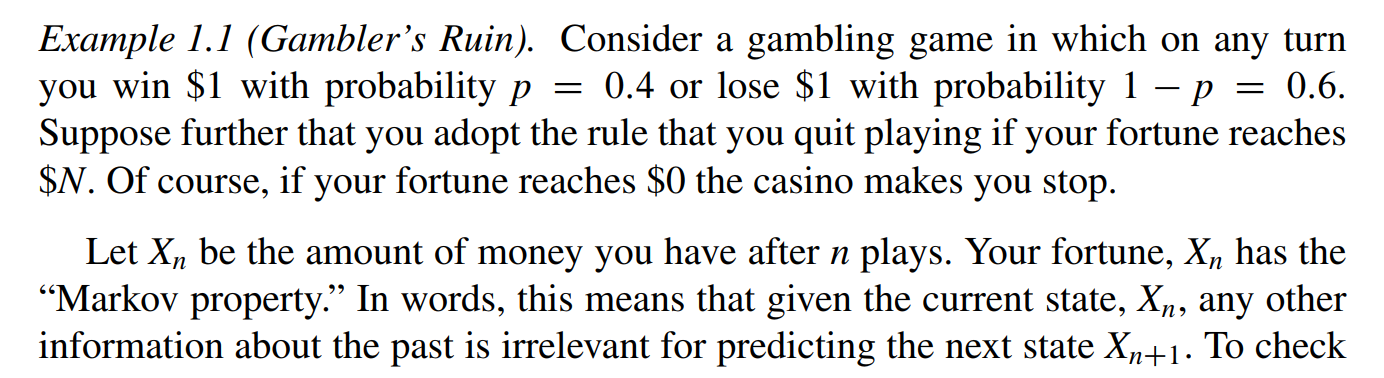
\includegraphics[width=0.9\textwidth]{figures/Gambler's Ruin.png}
        \caption{Gambler's Ruin}
    \end{figure}
\end{example}

$\{X_n,n\geq 0\}$ 为(时齐)马氏链

1. 对于 $0<i_0,\cdots,i_{n-1}<N, n\geq 0$ 有
\[
\begin{aligned}
    &\PP(X_{n+1}=i+1|X_n=i,X_0=i_0,\cdots,X_{n-1}=i_{n-1})\\
    =&\PP(X_{n+1}=i+1|X_n=i)=0.4=\PP(\text{第}n+1\text{次赌局赢一元})
\end{aligned}
\]
\[
\begin{aligned}
    &\PP(X_{n+1}=i-1|X_n=i,X_0=i_0,\cdots,X_{n-1}=i_{n-1})\\
    =&\PP(X_{n+1}=i-1|X_n=i)=0.6=\PP(\text{第}n+1\text{次赌局输一元})
\end{aligned}
\]